\section{Módulos}

\begin{definition}
O \emph{módulo} (ou \emph{valor absoluto}) de um número real $x$,
denotado por $\modu x$, é definido por:
%
$$
\modu x =
\begin{cases}
x , & \text{se $x \ge 0$} \\
-x, & \text{se $x<0$}.
\end{cases}
$$
\end{definition}

\noindent Para resolver equações modulares, usaremos dois métodos:
%
\begin{itemize}
  \item Eliminação do módulo pela definição; e/ou
  \item Partição em intervalos.
\end{itemize}

\begin{example}
Resolva as equações
\begin{enumerate}[(a)]
  \item $\modu {2x-5} = 3$;
  \item $\modu{2x-3} = 1-3x$;
  \item $\modu{3-x} - \modu{x+1} = 4$.
\end{enumerate}
\end{example}

\begin{solution}
\begin{enumerate}[(a)]
	\item[]
	\item Usaremos o método de eliminação do módulo pela definição. Note que:
	%
	\begin{align*}
		\modu{2x-5} = 
		\begin{cases}
		2x-5,    & \text{se } 2x-5 \ge 0 \iff x \ge 5/2 \\
		-(2x-5), & \text{se } 2x-5 < 0 \iff x < 5/2
		\end{cases}
	\end{align*}
	%
	Se $x \ge 5/2$, teremos:
	%
	\begin{align*}
	\modu{2x-5}=3 &\iff 2x-5=3 \\
				  &\iff x=4
	\end{align*}
	%
	Como $x=4\ge5/2$, temos que $4 \in S$.

	Se $x<5/2$, teremos:
	%
	\begin{align*}
		\modu{2x-5}=3 &\iff -\prn{2x-5} = 3 \\
					  &\iff -2x = -2 \\
					  &\iff x = 1 
	\end{align*}
	%
	Como $x=1<5/2$, então $1 \in S$.

	Das análises dos dois casos, concluímos que o conjunto solução é $S=\set{1,4}$.

	\item Novamente, usaremos o método de eliminação do módulo pela definição. Observe que:
	%
	\begin{align*}
		\modu{2x-3}= 
		\begin{cases}
			2x-3,    & \text{se } 2x-3 \ge 0 \iff x \ge \frac 3 2 \\
			-(2x-3), & \text{se } 2x-3 < 0 \iff x < \frac 3 2
		\end{cases}
	\end{align*}
	%
	Se $x \ge 3/2$, teremos:
	%
	\begin{align*}
		\modu{2x-3}=1-3x &\iff 2x-3=1-3x \\
						 &\iff x = \frac 4 5
	\end{align*}
	%
	Como $4/5 < 3/2$, então $4/5 \notin S$.

	Se $x < 3/2$, teremos:
	%
	\begin{align*}
		\modu{2x-3}=1-3x &\iff -\prn{2x-3}=1-3x \\
						 &\iff x = -2
	\end{align*}
	%
	Como $-2 < 3/2$, então $-2 \in S$.

	Das análises dos dois casos, concluímos que o conjunto solução é $S=\set{-2}$.

	\item Usaremos o método de partição em intervalos. Note que:
	%
	\begin{align*}
		& \modu{3-x}= 
		\begin{cases}
			3-x,    & \text{se } 3-x \ge 0 \iff x \le 3 \\
			-(3-x), & \text{se } 3-x < 0 \iff x > 3
		\end{cases}\\
		& \modu{x+1}= 
		\begin{cases}
			x+1,    & \text{se } x+1 \ge 0 \iff x \ge -1 \\
			-(x+1), & \text{se } x+1 < 0 \iff x < -1
		\end{cases}
	\end{align*}
	%
	\begin{itemize}
		\item Caso $x<-1$: 
		%
		\begin{align*}
			\modu{3-x}-\modu{x+1}=4 &\iff 3-x-\left[-(x+1)\right]=4\\
									&\iff 4=4 \ \ \ \text{ para todo } x \in \R
		\end{align*}
		%
		Temos, então, que $x<-1$ é solução para a equação.
		%
		\item Caso $-1 \le x \le 3$:
		%
		\begin{align*}
			\modu{3-x}-\modu{x+1}=4 &\iff 3-x-(x+1)=4\\
									&\iff -2x+2=4\\
									&\iff x=-1
		\end{align*}
		%
		Logo, $x=-1$ é solução da equação.
		%
		\item Caso $x>3$:
		%
		\begin{align*}
			\modu{3-x}-\modu{x+1}=4 &\iff -(3-x)-(x+1)=4\\
									&\iff -4=4
		\end{align*}
		%
		Nesse caso, não há soluções.
	\end{itemize}

	Das análises dos casos, conclui-se que $S=\set{x \in \R \tq x \le -1}$.
\end{enumerate}
\end{solution}

\begin{onlineact}
	\khan{https://pt.khanacademy.org/math/algebra-home/alg-absolute-value/alg-absolute-value-equations/e/absolute_value_equations}{Resolva Equações Modulares}.
\end{onlineact}

\begin{proposition}[Propriedades de inequações modulares]
Sejam $x \in \R$, $a\in \R^*_+ $.
%
\begin{enumerate}
  \item $\modu x \geq 0$;
  \item $\modu x < a \Leftrightarrow -a < x < a$;
  \item $\modu x > a \Leftrightarrow x > a$ ou $x < -a$;
  \item $-\modu x \leq x \leq \modu x$.
\end{enumerate}
%
Os resultados (ii) e (iii) também são válidos para os casos com $\le$ e $\ge$, respectivamente.
\end{proposition}

\begin{tve}
    \link{https://drive.google.com/file/d/1HK3Jujp4h4VNOep-6djEYm6CH0zIRxgn/view?usp=sharing}{Propriedades de inequações modulares}
\end{tve}

\begin{example}
Resolva as inequações:
%
\begin{enumerate}[(a)]
  \item $\modu {2x-5} < 3$;
  \item $\modu{2x-3} \geq 1-3x$;
  \item $\modu{3-x} - \modu{x+1} \leq 4$.
\end{enumerate}
\end{example}

\begin{solution}
\begin{enumerate}[(a)]
	\item[]
	\item Exercício.
	\item Exercício.
	\item Usaremos novamente o método da partição em intervalos. Note que:
	%
	\begin{align*}
		& \modu{3-x}= 
		\begin{cases}
			3-x,    & \text{se } 3-x \ge 0 \iff x \le 3 \\
			-(3-x), & \text{se } 3-x < 0 \iff x > 3
		\end{cases}\\
		& \modu{x+1}= 
		\begin{cases}
			x+1,    & \text{se } x+1 \ge 0 \iff x \ge -1 \\
			-(x+1), & \text{se } x+1 < 0 \iff x < -1
		\end{cases}
	\end{align*}

	\begin{itemize}
		\item Caso $x<-1$:
		%
		\begin{align*}
			\modu{3-x}-\modu{x+1}\le4 & \iff 3-x-\left[-\prn{x+1}\right]\le 4\\
									  & \iff 4 \le 4 \ \ \ \ \text{para todo } x \in \R
		\end{align*}
		%
		A interseção das restrições para este caso é calculada na Figura \ref{fig:08-28-cut1}.
		%
		\begin{figure}[H]
		\caption{}
		\label{fig:08-28-cut1} % LABEL MUST APPEAR AFTER CAPTION!
		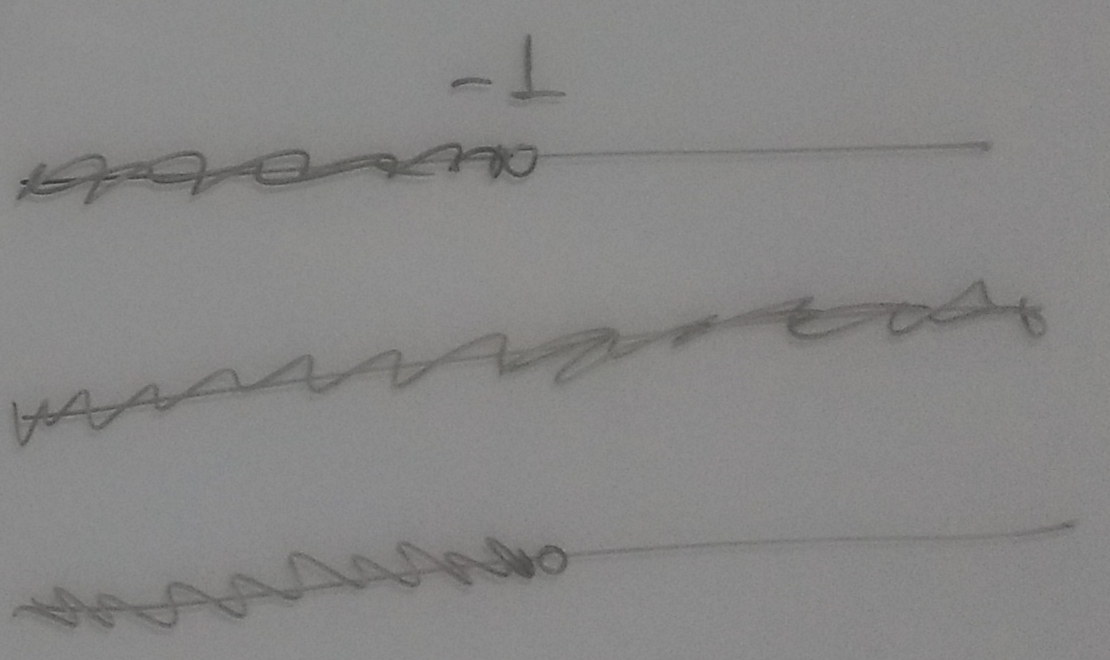
\includegraphics[scale=0.3]{\imgdirfromsection/cut1.jpg}
		\centering
		\end{figure}
		%
		Da figura, conclui-se que $x<-1$ é solução para a inequação.
		%
		\item Caso $-1 \le x \le 3$:
		%
		\begin{align*}
		\modu{3-x} - \modu{x+1} \le 4 & \iff 3-x-\prn{x+1} \le 4 \\
		& \iff -2x+2\le 4\\ 
		& \iff x \ge -1
		\end{align*}
		%
		A interseção das restrições para este caso é calculada na Figura \ref{fig:08-28-cut2}.
		%
		\begin{figure}[H]
		\caption{}
		\label{fig:08-28-cut2} 
		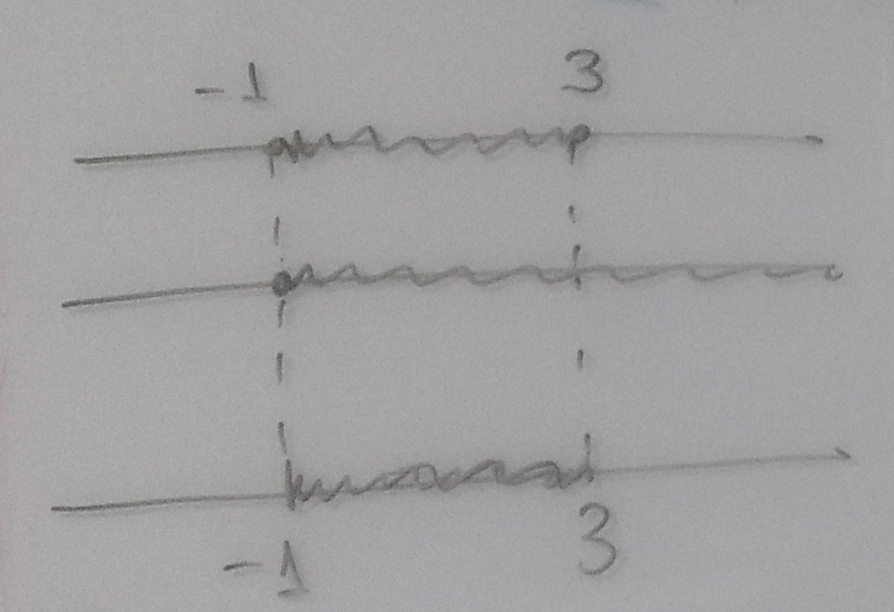
\includegraphics[scale=0.3]{\imgdirfromsection/cut2.jpg}
		\centering
		\end{figure}
		%
		Pela figura, conclui-se que $-1 \le x \le 3$ é solução para a inequação.
		%
		\item Caso $x > 3$:
		%
		\begin{align*}
		\modu{3-x} - \modu{x+1} \le 4 & \iff -\prn{3-x}-\prn{x+1} \le 4 \\
		& \iff -4\le 4 \text{ para todo }x \in \R
		\end{align*}
		%
		Na Figura \ref{fig:08-28-cut3}, é calculada a interseção das restrições para este caso.
		%
		\begin{figure}[H]
		\caption{}
		\label{fig:08-28-cut3} 
		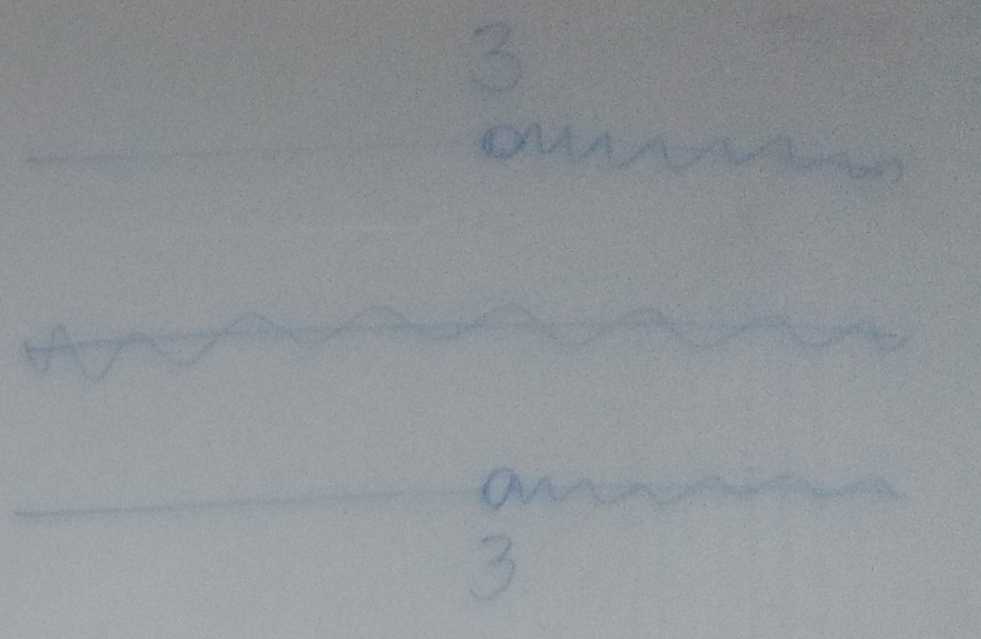
\includegraphics[scale=0.3]{\imgdirfromsection/cut3.jpg}
		\centering
		\end{figure}
		%
		A partir da análise da figura, conclui-se que $x>3$ também é solução para a inequação.
	\end{itemize}
\end{enumerate}
%
Na Figura \ref{fig:08-28-cut4}, é calculada a união das soluções de todos os casos.
%
\begin{figure}[H]
\caption{}
\label{fig:08-28-cut4} 
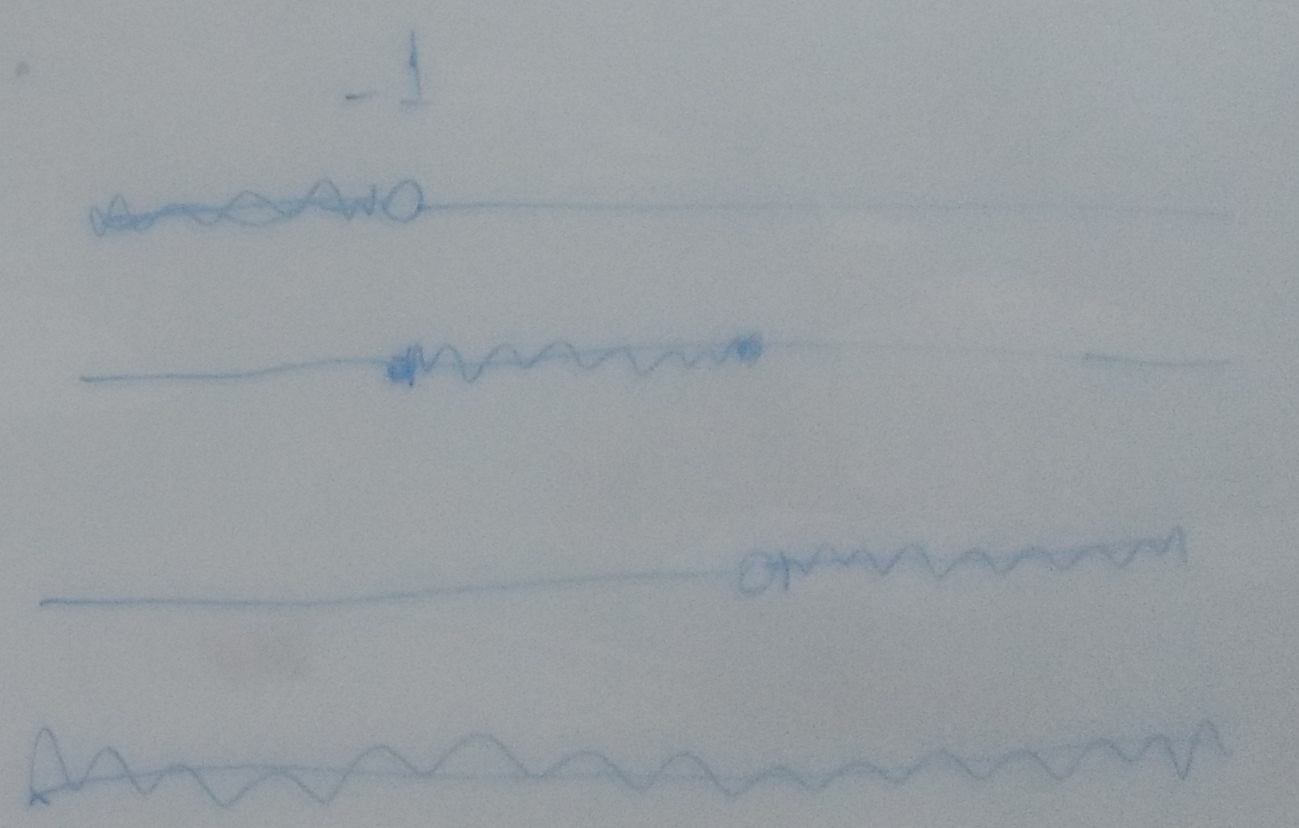
\includegraphics[scale=0.3]{\imgdirfromsection/cut4.jpg}
\centering
\end{figure}
%
Das análises dos três casos e da figura, pode-se concluir que o conjunto solução da inequação é o próprio conjunto dos números reais.
\end{solution}